\documentclass[11pt]{article}
\usepackage{spikey}
\usepackage{amsmath}
\usepackage{amssymb}
\usepackage{soul}
\usepackage{float}
\usepackage{graphicx}
\usepackage{hyperref}
\usepackage{xcolor}
\usepackage{chngcntr}
\usepackage{mathrsfs}
\usepackage{centernot}
\usepackage[shortlabels]{enumitem}
\usepackage{verbatim}

\usepackage[margin=1truein]{geometry}
\usepackage{setspace}
\linespread{1.0}

\title{Analysis on PANSS Dataset\\ \small STATS 202: Data Mining and Analysis, Final Project}
\author{Tianyu Du}
\date{\today}

\begin{document}
	\maketitle
	\tableofcontents
%	\newpage

	\section{Introduction}
%	\subsection{PANSS Dataset}
	\paragraph{}The Positive and Negative Syndrome Scale (PANSS) score is widely used as a measure for schizophrenia and other disorders in clinical trials. PANSS scores are collected by trained raters and reported by patients or their relatives. One assessment of PANSS scores consists 30 sub-scores from 3 sub-categories: 7 positive scores, 7 negative scores, and 16 general scores. Every score ranges from 1 to 7 denoting increasing levels of psychopathology. The aggregation of all 30 scores provides a detailed assessment of patient's current psychological status.
	
	\paragraph{}The entire dataset consists of five different studies ranging from study A to study E. In this practice, the first four datasets are used as a training to fit, select, and evaluate models. Then, these selected models are used to recover missing data in study E.
	
	\section{Treatment Effects}
	\paragraph{}This section is devoted to analyze whether the treatment assigned leads to significant improvements on patients' psychological status. Because the 18-th week assessments are missing in the dataset of study E, in this section, only data from study A to D are considered. There are 20947 observations (assessments) from above-mentioned dataset, in which 10524 observations came from patients assigned to the control group, and the remaining 10423 were from participants belonged to the treatment group. The evenly-split dataset allows us to deploy various models to analyze whether there exists significant treatment effects.
	
	\paragraph{}Multiple evidences were found to support that there were indeed no treatment effect in this study. Firstly, the effects on four aggregate scores are analyzed, namely sum of all PANSS scores, and sums of scores from positive (\texttt{P\_Total}), negative (\texttt{N\_Total}), and general (\texttt{G\_Total}) sub-categories respectively.
	
	\paragraph{}One challenge associated with treatment effect analysis is the initial status of patients in different groups. In some cases, the \emph{prior} psychological status for a randomly selected patient from the treatment group is expected to be different from that of a random patient in the control group. In these cases, even if significant differences in PANSS scores \emph{posterior} to the treatment were supported, one will not be able to distinguish whether the "effect" came from the discrepancy in the prior distributions or the treatment, and the treatment effect is not well-identifies.
	Figure 1 below presents the distributions of the four aggregate scores at day 0 visit. Both groups shared similar histograms in terms of all four metrics. Moreover, the estimated kernel densities collided, which provided further evidence that there were no significant prior discrepancies between patients from these two groups. Therefore, one can conclude that most posterior differences in PANSS metrics were resulted from the treatment assigned.

	\begin{figure}[H]
		\centering
		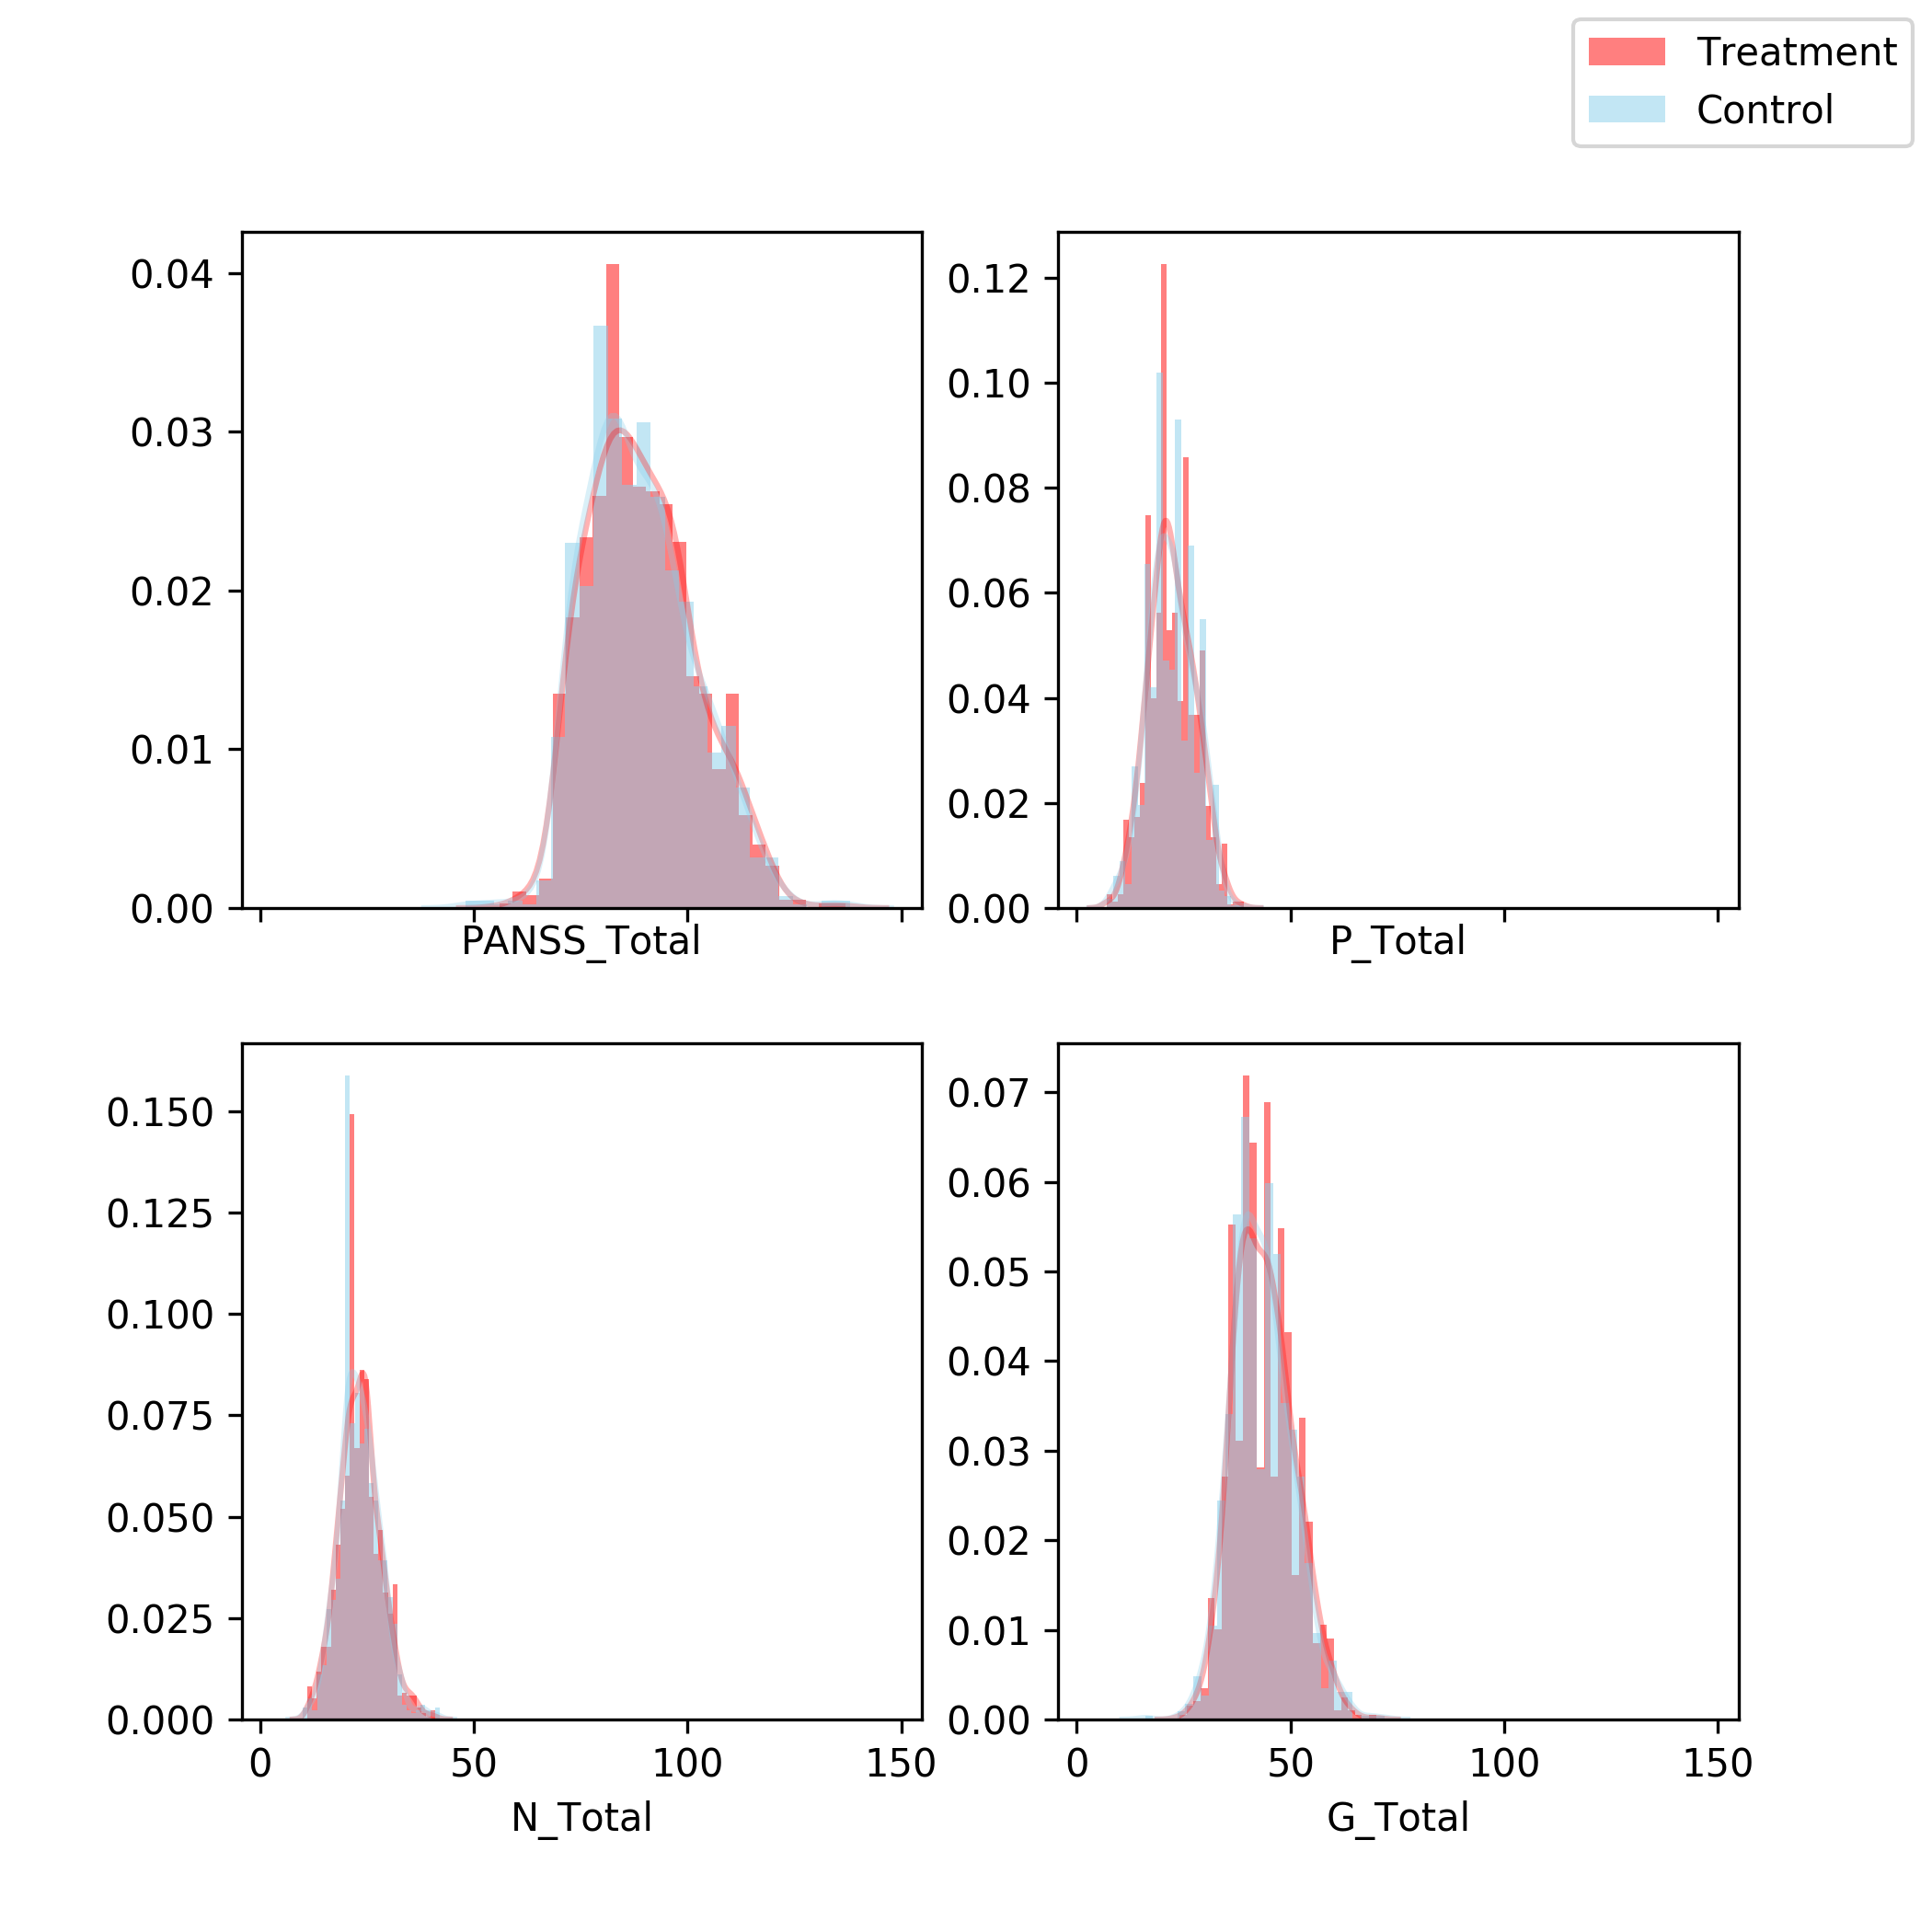
\includegraphics[width=0.7\linewidth]{figures/dist_initial_scores.png}
		\caption{Distributions of Aggregate Scores at Day 0}
	\end{figure}

	\paragraph{}The evolving path of these four above mentioned metrics can provide reasonable proxies to the treatment effect. As mentioned before, we believed the data failed to provide sufficient evidence to support the existence of treatment effect. Let $t \in \N$ denote the \texttt{VisitDay} variable in the dataset, $t$ ranges from 0 to 480 in the complete dataset. Figure 2 presents the distribution of $t$, the 95-percent quantile is located at $t_{95\%} = 297$. Therefore, the top 5\% of observations occupied more than on third of the total range of $t$, these observations are potentially troublesome as outliers. To deal with this issue, the top 5\% observations are excluded from following analysis.

	\begin{figure}[H]
		\centering
		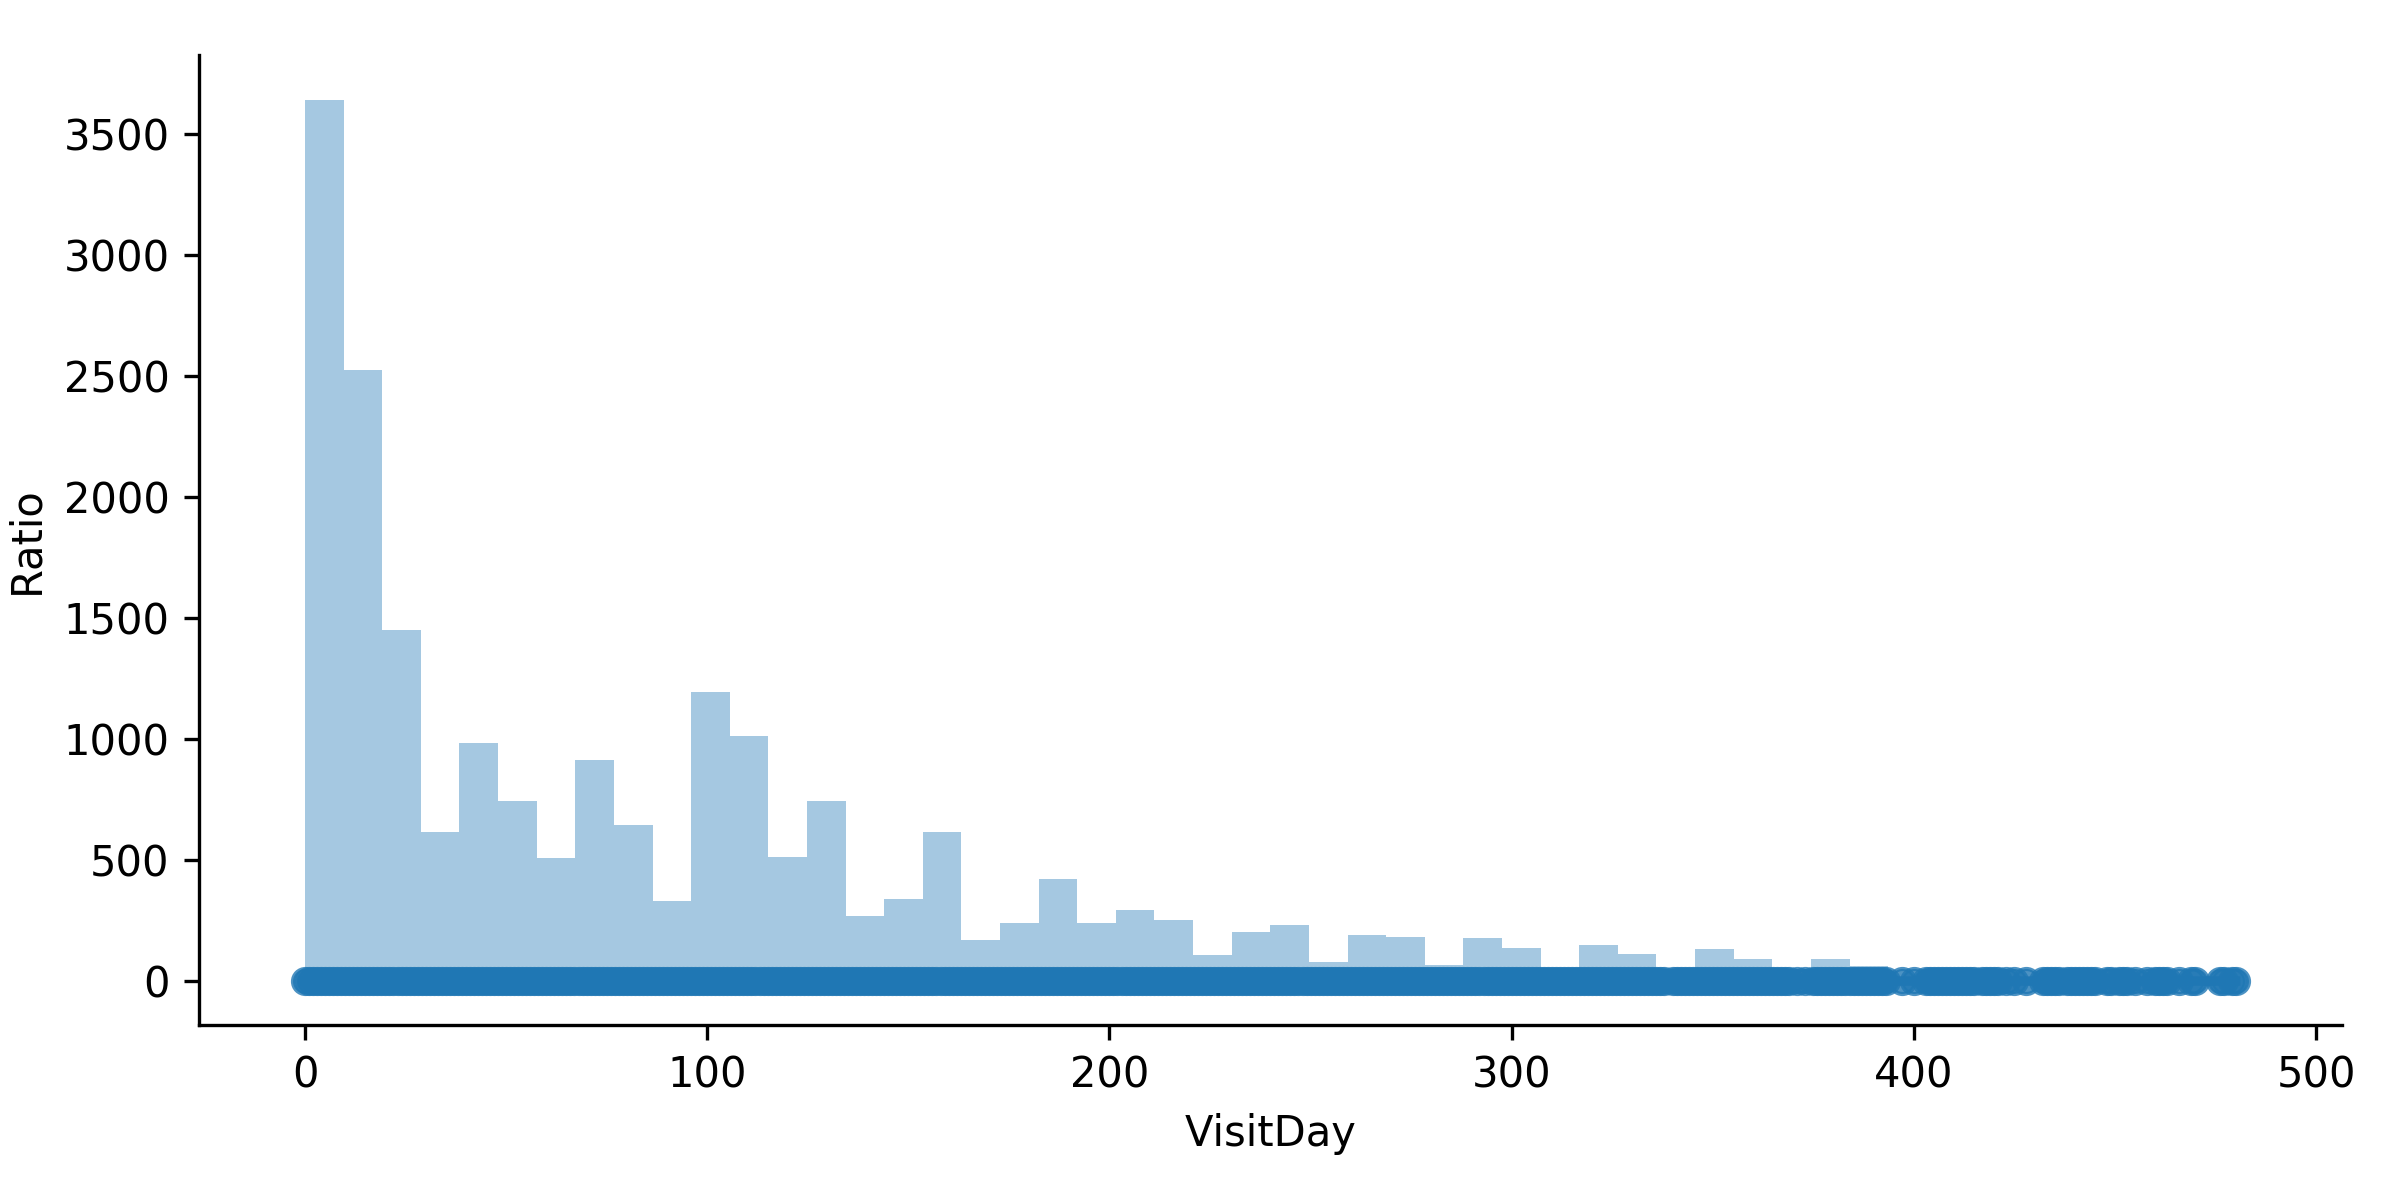
\includegraphics[width=0.7\linewidth]{figures/dist_visit_day_all.png}
		\caption{Distribution of \texttt{VisitDay}}
	\end{figure}
	
	\paragraph{}The general strategy to identify treatment effect here uses linear models. Let $Y$ denote the target metric, which takes value from the four aggregate PANSS metrics: $\mc{M} := \{ \Sigma_{PANSS}, \Sigma_P, \Sigma_N, \Sigma_G\}$. Let $X$ denote the set other characteristics of the patient. And a hybrid linear model is fit:
	\begin{align}
		Y &= f_0(X, t) + \id{\texttt{Treatment}} f_1(X, t)
	\end{align}
	where $f_0$ and $f_1$ are two additive linear models, so that $f_0$ captures the evolving path of $Y$ over time for the population of the control group, and the additive term $f_1$ measures the discrepancy of the treatment group.
	Should the treatment dummy variable is statistically significant, then one can conclude the existence of treatment effect.
	\subsection{Patterns of PANSS over Time}
	\paragraph{}Figure 3 below shows the scatter plot of $\Sigma_{PANSS}$ scores against time for both groups with corresponding locally weighted linear regression estimations (LOWESS). The LOWESS for the treatment and control groups almost collide perfectly, which means the trends for both group estimated from non-parametric model are essentially identical, this provides preliminary evidence supporting our claim that there was no significant treatment effect.
	\begin{figure}[H]
		\centering
		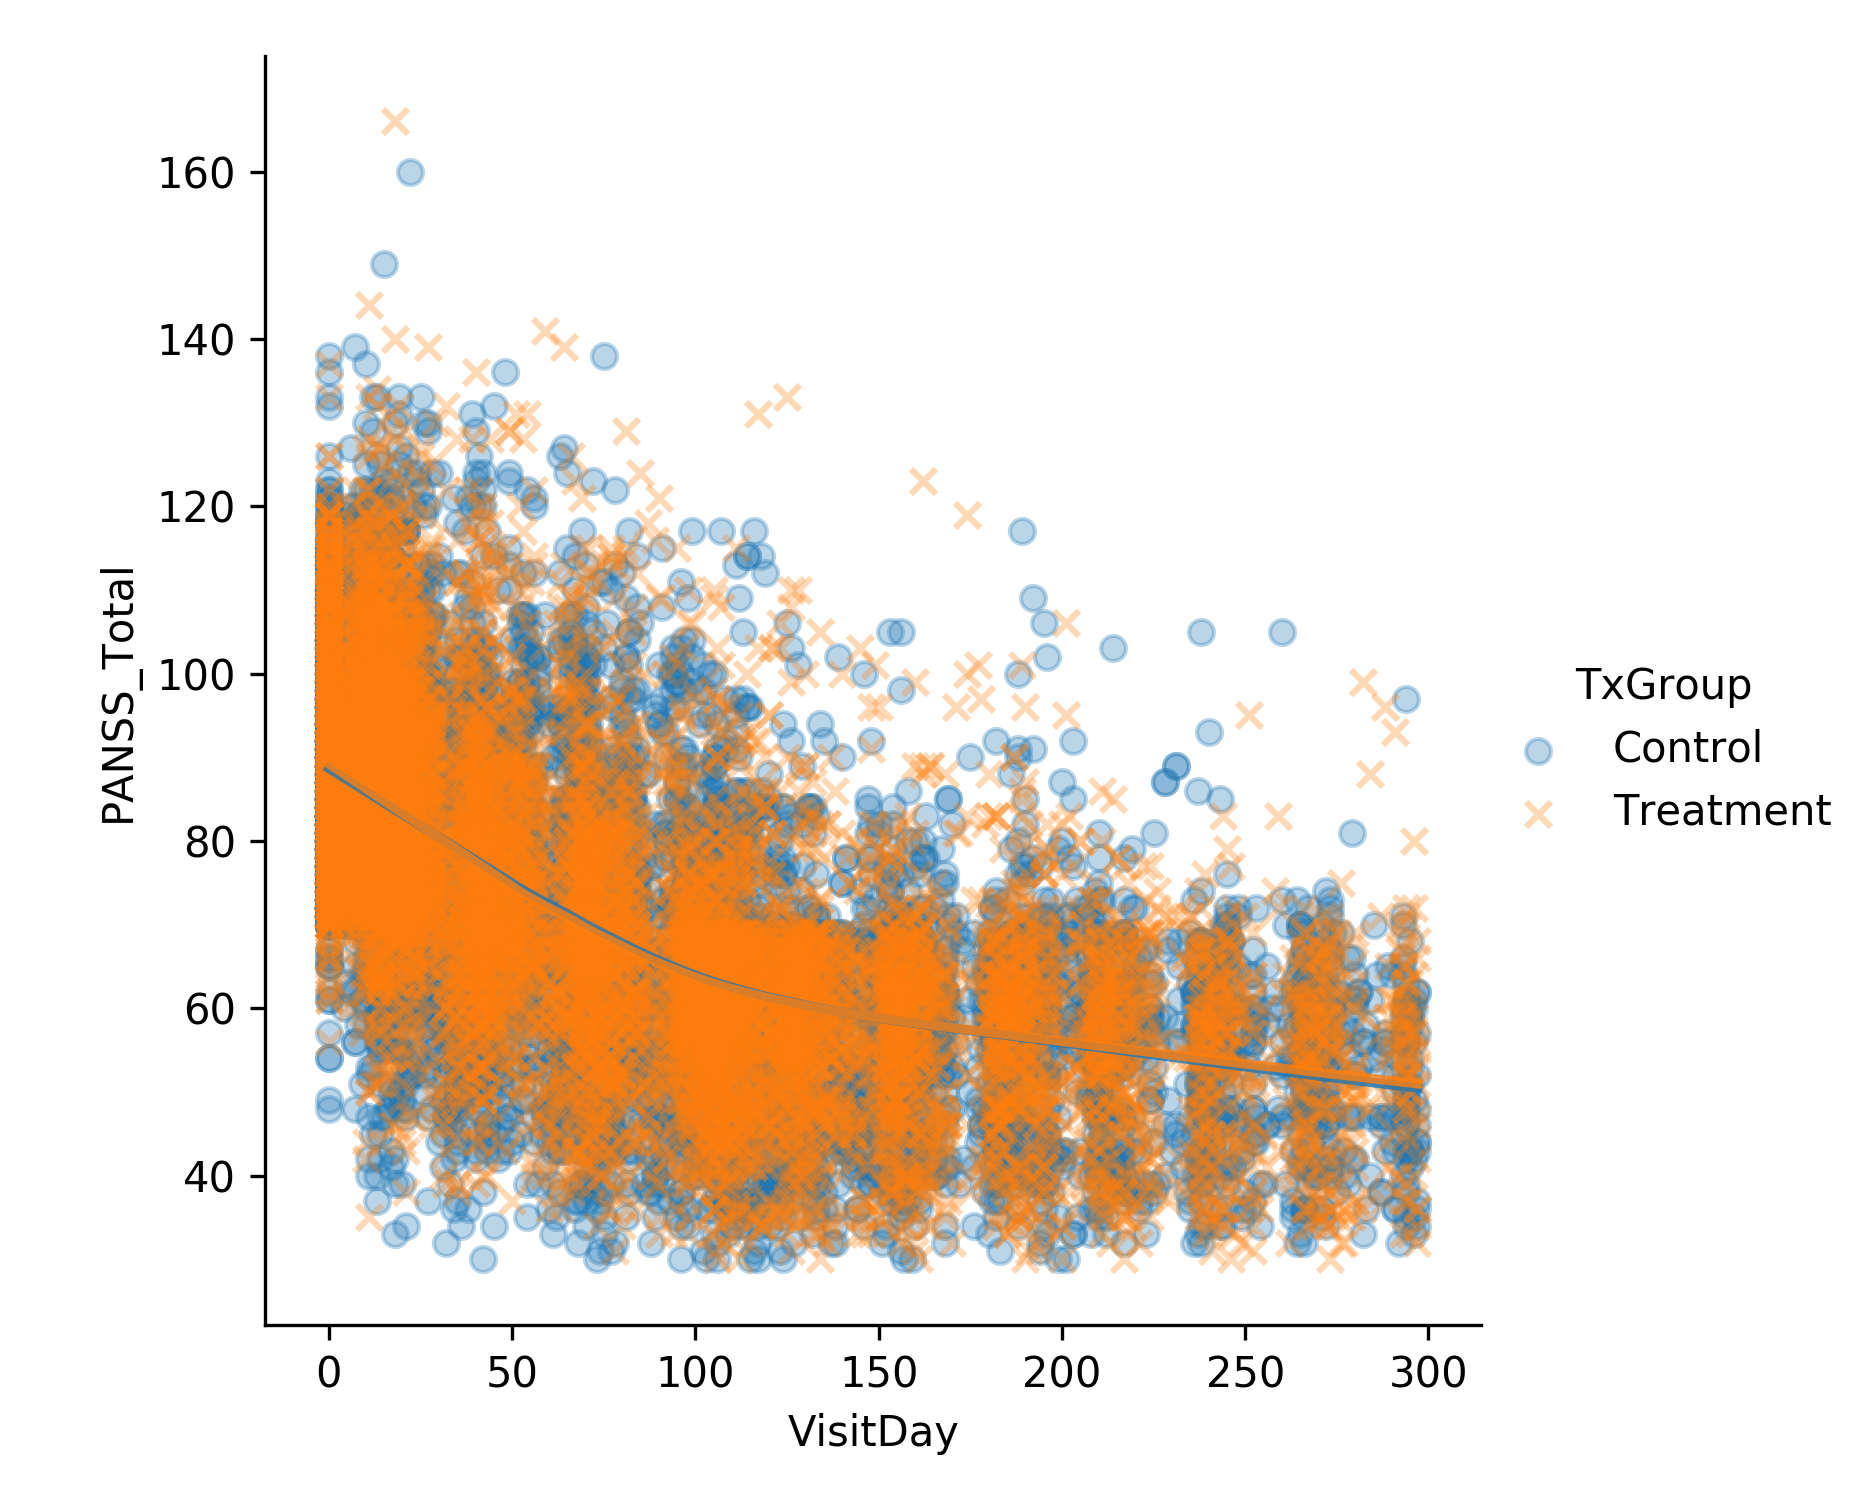
\includegraphics[width=0.7\linewidth]{figures/lwlm_te_PANSS_Total.png}
		\caption{Changes of \texttt{PANSS\_Total} Over Time and LOWESS}
	\end{figure}
	\subsection{Identifying Treatment Effect with Hypothesis Testing}
	\paragraph{} As the plot in figure 3 suggests, the relationship between PANSS scores and $t$ is more or less quadratic. Moreover, similar quadratic characteristics were also found on the other three aggregate metrics (see appendix). Therefore, $f_0$ and $f_1$ are identified as quadratic functions of $t$, specifically,
	\begin{align}
		Y &= f_0(X, t) + \id{\texttt{Treatment}} f_1(X, t) \\
		&= \left(\beta_{0, 0} + \beta_{0, 1} t + \beta_{0, 2} t^2 + \vec{\gamma}_0 \texttt{Country} + \vec{\delta}_0 \texttt{Study}\right) \\
		&+ \id{\texttt{Treatment}} \left(\beta_{1, 0} + \beta_{1, 1} t + \beta_{1, 2} t^2 + \vec{\gamma}_1 \texttt{Country} + \vec{\delta}_1 \texttt{Study}\right) + \varepsilon \\
		&= \theta_0 + \theta_1 t + \theta_2 t^2 + \theta_3 \id{\texttt{Treatment}} + \theta_4 \id{\texttt{Treatment}} t + \theta_5 \id{\texttt{Treatment}} t^2 + \\
		&+\vec{\gamma}_0 \texttt{Country} + \vec{\delta}_0 \texttt{Study} + Z + \varepsilon
	\end{align}
	where $\texttt{Study}$ and $\texttt{Country}$ denote the collection of dummy variables, and $Z$ denotes the set of interaction terms between variables in $X$ and $\id{\texttt{Treatment}}$. It could be controversial whether to include interacting terms between $\id{\texttt{Treatment}}$ and variables other than $t$. As a result, p-values under all combination of optional covariates are reported.
	
	\begin{table}[H]
	\centering
	\begin{tabular}{l|c|c|c|c}
		Covariates from $Z$ & $\varnothing$ & \texttt{C}*\texttt{T} & \texttt{S}*\texttt{T} & \texttt{C}*\texttt{T} + \texttt{S}*\texttt{T}\\
		\hline
		\texttt{PANSS\_Total} $\sim$ \texttt{T}& $0.5167(0.1873)^{**}$& -2.113(1.577)& & \\
		\texttt{PANSS\_Total} $\sim$ $\texttt{T} \times t$ & -35.95(26.40)& -31.33(26.91)& & \\
		\texttt{PANSS\_Total} $\sim$ $\texttt{T} \times t^2$ & 24.99 (26.36) & 23.72(26.36)& & \\
		\hline 
		\texttt{P\_Total} $\sim$ \texttt{T}& 0.06806(0.06473)&  & & \\
		\texttt{P\_Total} $\sim$ $\texttt{T} \times t$ & -7.643(9.121) & & & \\
		\texttt{P\_Total} $\sim$ $\texttt{T} \times t^2$ & 14.65(9.107)& & & \\
		\hline
		\texttt{N\_Total} $\sim$ \texttt{T}& 0.1132(0.06793)$^\dagger$&  & & \\
		\texttt{N\_Total} $\sim$ $\texttt{T} \times t$ & -10.22(9.571)& & & \\
		\texttt{N\_Total} $\sim$ $\texttt{T} \times t^2$ & 0.4369(9.557)& & & \\
		\hline
		\texttt{G\_Total} $\sim$ \texttt{T}&  0.3353(0.09998)$^{***}$&  & & \\
		\texttt{G\_Total} $\sim$ $\texttt{T} \times t$ & -18.09(14.09) & & & \\
		\texttt{G\_Total} $\sim$ $\texttt{T} \times t^2$ & 9.901 (14.07)& & & \\
	\end{tabular}
	\caption{Regression Results with Different Combination of Variables (standard error)}
	\end{table}

	
	\section{Patient Segmentation}
	\section{Patient PANSS Forecasting}
	\section{Assessment Validity Classification}
	
	\section{Appendix}
\end{document}










